\documentclass[svgnames,tikz]{standalone}
\usetikzlibrary{positioning,arrows.meta,calc}
\usepackage{lmodern}


\tikzset{
   class/.style={draw, fill=LightYellow},
   template/.style={label={[mTemplateNodeStyle]north east:#1}},
   realization/.style={-Latex[open]},
%%
   mTemplateNodeStyle/.style={fill=white,draw,dashed,font={\tt\small}, inner sep=2pt, anchor=center}
}


\begin{document}
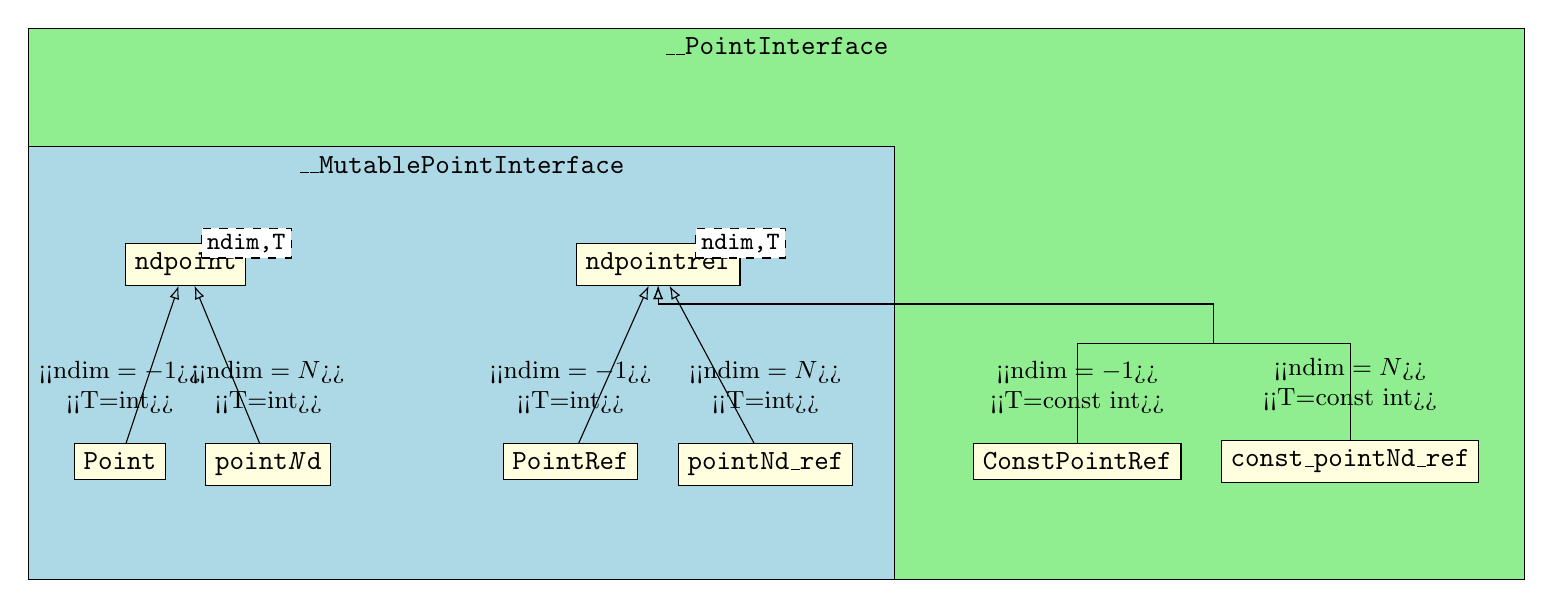
\begin{tikzpicture}[
  every node/.style={font=\tt},
  edge from parent path={[latex-] (\tikzparentnode.south) -- ++(0,-.5) -| (\tikzchildnode)}
  ]

  \draw[fill=LightGreen] (-5,1) rectangle (14,-6);
  \node[align=center,below] (PI) at (4.5,1) {\_\_PointInterface\\};


  % \node (CPR) at (5,-2) {pointref<ndim, const T>};

  \draw[fill=LightBlue] (-5,-.5) rectangle (6,-6);
  \node[align=center,below] (PI) at (0.5,-.5) {\_\_MutablePointInterface\\};


  \node[class, template={ndim,T}] (ndpoint) at (-3,-2){ndpoint};
  \node[class, template={ndim,T}] (ndpointref) at (+3,-2){ndpointref};

  \node[class, below left=2cm and 0.25cm of ndpoint.south] (Point){Point};
  \node[class, below right=2cm and 0.25cm of ndpoint.south, name=pointnd] (pointnd){point\emph{N}d};


  \draw[realization] (Point) -- (ndpoint);
  \draw[realization] (pointnd) -- (ndpoint);

  \node[above=0.25cm of Point, font=\small, align=center] { <<$\mathrm{ndim}=-1$>>\\ <<T=int>> };
  \node[above=0.25cm of pointnd, font=\small, align=center] { <<$\mathrm{ndim}=N$>>\\ <<T=int>> };


  \node[class,below left=2cm and 0.25cm of ndpointref.south] (PointRef) {PointRef};
  \node[class,below right=2cm and 0.25cm of ndpointref.south] (pointndref) {pointNd\_ref};
  \draw[realization](PointRef) -- (ndpointref);
  \draw[realization](pointndref) -- (ndpointref);
  \node[above=0.25cm of PointRef, font=\small, align=center] { <<$\mathrm{ndim}=-1$>>\\ <<T=int>> };
  \node[above=0.25cm of pointndref, font=\small, align=center] { <<$\mathrm{ndim}=N$>>\\ <<T=int>> };

  \node[class,below right=2cm and 4cm of ndpointref.south] (ConstPointRef) {ConstPointRef};
  \node[class,right=0.5cm of ConstPointRef] (constpointndref) {const\_pointNd\_ref};

  \coordinate (U) at ($ (ConstPointRef)!0.5!(constpointndref) + (0,1.5) $);
  \draw[realization](ConstPointRef) |- (U) -- ++(0,0.5) -| (ndpointref);
  \draw[realization](constpointndref) |- (U) -- ++(0,0.5) -| (ndpointref);
  \node[above=0.25cm of ConstPointRef, font=\small, align=center] { <<$\mathrm{ndim}=-1$>>\\ <<T=const int>> };
  \node[above=0.25cm of constpointndref, font=\small, align=center] { <<$\mathrm{ndim}=N$>>\\ <<T=const int>> };


  % \draw [latex-] (PI.340) -- ++(0,-.5) -| (CPR);



  \end{tikzpicture}
\end{document}